\documentclass[../Hovedrapport.tex]{subfiles}
\begin{document}
%\vspace{-30pt}
%------------------------------------------------------------------------------
\section{Dimensionering af fordamper}
    \label{sec:dim_fordamper}

Fordamperen ønskes dimensioneret på en sådan måde, at den kan optage en varme i køleskabet svarende til den maksimale kuldeydelse på $\SI{334}{W}$ som kompressoren kan levere ved dens maksimale omdrejningstal $\SI{4000}{rpm}$. Ligeledes ønskes fordamperen konstrueret sådan, at den kan optage den mængde varme, svarende til den kuldeydelse på $\SI{222}{W}$ kompressoren kan yde ved laveste omdrejningstal der er $\SI{2500}{rpm}$.\citep{Coolselector_BD350GH}

På nedstående skitse ses betegnelser for, hvor eksempelvis de tværgående rør er målt. Skitsen er ikke målfast men har til formål at skabe et overblik over betegnelserne i tabel \ref{tab:Fordamper_Data}.
% --- Her skal der indsættes en skitse omkring fordamperen, som Jeppe har tegnet ---

\begin{figure}[H] % Fordamper forside
	\centering
	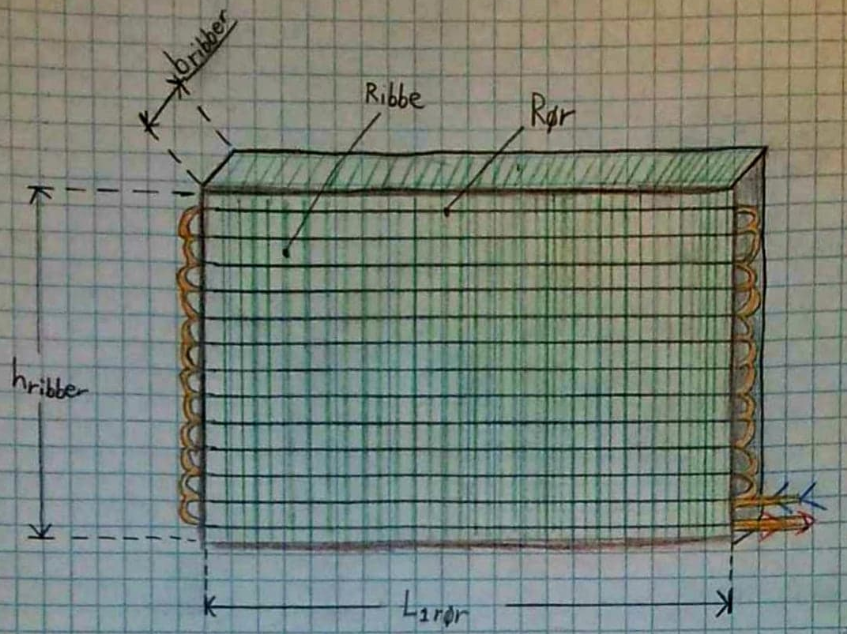
\includegraphics[width=0.9\textwidth]{Billeder/fordamper_forside.PNG}
	\caption{\textit{Her ses fordamperen forfra.}}
	\label{fig:fordamp_forside}
\end{figure}

\begin{figure}[H] % Fordamper side
	\centering
	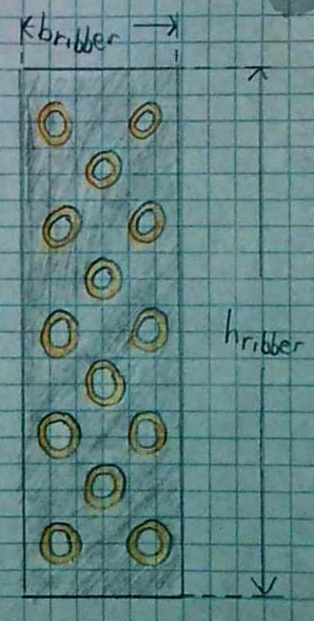
\includegraphics[width=0.4\textwidth]{Billeder/fordamper_side.PNG}
	\caption{\textit{Her ses en princip tegning af, hvordan rørføringen er igennem fordamperen. Tegningen viser fordamperen fra siden.}}
	\label{fig:fordamp_forside}
\end{figure}

\begin{figure}[H] % Fordamper roer
	\centering
	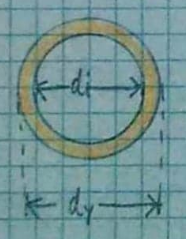
\includegraphics[width=0.3\textwidth]{Billeder/fordamper_roer.PNG}
	\caption{\textit{Her ses et tværsnit af et rør, som løber igennem fordamperen.}}
	\label{fig:fordamp_forside}
\end{figure}


\newpage

Data for lamelvarmeveksleren findes i nedstående tabel \ref{tab:Fordamper_Data}:


%------------------------------TABEL START----------------------------
\begin{table}[H] 
	\centering
	% \caption*{\textbf{\large Fordamper data}} 
	% \vspace{-0.3cm}
	\begin{tabular}{|c|l|l|c|}  \rowcolor[gray]{0.5}                                \hline
	\multicolumn{4}{|c|}{\textbf{Fordamper dimensioner}}                                                                       \\ \hline \rowcolor[gray]{.8}
	\textbf{Variabel}   & \textbf{Værdi}        & \textbf{Forklaring}       & \textbf{Kilde}                            \\ \hline \rowcolor[gray]{.95}
	L_\text{1rør}        & \SI{0,22}{\meter}     & Rørlængde af et tværgående rør i fordamper   & Målt                  \\ \hline \rowcolor[gray]{.95} 
	L_\text{rør}        & \SI{5,28}{\meter}     & Rørlængde i fordamper   & Målt                                        \\ \hline \rowcolor[gray]{.95} 
	d_\text{i}          & \SI{7}{\milli\meter}  & Indre rørdiameter         & Målt                                      \\ \hline \rowcolor[gray]{.95}
	d_\text{y}          & \SI{8}{\milli\meter}  & Ydre rørdiameter          & Målt                                      \\ \hline \rowcolor[gray]{.95}
	s_\text{q}          & \SI{25}{\milli\meter}  & Centerafstand mellem to rør lodret over hinanden        & Målt       \\ \hline \rowcolor[gray]{.95}
	s_\text{r}          & \SI{18}{\milli\meter}  & Centerafstand mellem to rør diagonalt ved siden af hinanden        & Målt              \\ \hline \rowcolor[gray]{.95}
	b_\text{ribber}     & \SI{0,037}{\meter}    & Ribbebredde               & Målt                                      \\ \hline \rowcolor[gray]{.95}
	h_\text{ribber}     & \SI{0,2}{\meter}      & Ribbehøjde                & Målt                                      \\ \hline \rowcolor[gray]{.95}
	t_\text{ribber}     & \SI{0,0001}{\meter}    & Ribbetykkelse             & Målt                                     \\ \hline \rowcolor[gray]{.95}
	N_\text{ribber}     & 71                    & Antallet af ribber        & Målt                                       \\ \hline \rowcolor[gray]{.95}
	N_\text{rørrækker}  & 3                     & Antallet af rørrækker     & Målt              \\ \hline \rowcolor[gray]{.95}
	N_\text{rør}        & 24                    & Antallet af rør           & Målt              \\ \hline \rowcolor[gray]{.95}
	N_\text{serie}      & 1                     & Antal fordampere i serie& Målt              \\ \hline \rowcolor[gray]{.5}
	\multicolumn{4}{|c|}{\textbf{Anlægsdata}}                                                   \\ \hline \rowcolor[gray]{.8}
	\textbf{Variabel}   & \textbf{Værdi}        & \textbf{Forklaring}       & \textbf{Kilde}    \\ \hline \rowcolor[gray]{.95}
	x_\text{g}          & 1                     & Dampkvalitet før fordamper - væske   & \\ \hline \rowcolor[gray]{.95}
	x_\text{L}          & 0                     & Dampkvalitet før kondensator - mættet gas & \\ \hline \rowcolor[gray]{.95}
	g                   & \SI{9,81}{m/s^2}      & Tyngdeaccelerationen                        & \\ \hline \rowcolor[gray]{.95}
	C                   & 0,41                  & Faktor c for fortsatte røranordning         & Aages noter \\ \hline \rowcolor[gray]{.95}   
	m                   & 0,60                  & Eksponent M for fortsatte røranordning      & Aages noter     \\ \hline \rowcolor[gray]{.95}
	t_\text{rk}         & \SI{50}{\celsius}     & Kondenseringstemperaturen                   & Antagelse       \\ \hline \rowcolor[gray]{.95}
	t_\text{L,1}        & \SI{7}{\celsius}      & Lufttemperaturen før fordamperen              & Antagelse     \\ \hline \rowcolor[gray]{.95}
	t_\text{L,2}        & \SI{3,6}{\celsius}    & Lufttemperaturen efter fordamperen            & Antagelse     \\ \hline \rowcolor[gray]{.95}
    t_\text{R1}         & \SI{-8}{\celsius}     & Kølemiddlets temperatur før fordamperen        & Antagelse    \\ \hline \rowcolor[gray]{.95}
	t_\text{R1}         & \SI{-8}{\celsius}     & Kølemiddlets temperatur efter fordamperen        & Antagelse  \\ \hline \rowcolor[gray]{.95}
	\end{tabular} 
	\caption{\textit{Variabeloversigt til dimensionering af fordamperen}} 
	\label{tab:Fordamper_Data} 
	\vspace{-20pt}
\end{table} \\ \\


% Vi bør overveje om temperaturen ikke skal estimere til 4 degC fordi det er nermere den man vil have i et køleskab. jo men så skal der jo ikke køles noget ned.
I beregningerne bliver temperaturer inde i køleskabet  sat til $\SI{7}{\celsius}$. Temperaturen bliver valgt grundet der ønskes at fordamperen er i stand til at køle køleskabet ned med fuld kuldeydelse, når temperaturen overstiger $\SI{4}{\celsius}$, der er den ønskede temperatur i køleskabet. Her antages det at når temperaturen når $\SI{7}{\celsius}$, vil køleskabet opleve en maksimal indre temperatur. % Skal der skrives en dybere forklaring her?.


Luftens temperatur efter den er suget igennem fordamperen af blæseren gættes i første omgang, og er senere bestemt, gennem iterativ process, til $\SI{3,6}{\celsius}$. Dette er ved at DC kompressoren kører med 4000 rpm, som er det højeste omdrejningstal den kan køre med. Når temperaturen falder under  $\SI{7}{\celsius}$, så falder kompressorens omdrejningshastighed også. Dette er kompressoren programeret til, for at sikre en stabil køling af indholdet i køleskabet.


Det antages at kølemiddlet har konstant temperatur igennem fordamperen. Derfor bliver antagelsen at kølemiddlet har fordampningstemperaturen på $\SI{-8}{\celsius}$ igennem hele fordamperen. Her ses der fort fra overhedningen på $\si{8}{\celsius}$.
\begin{align}
    t_{R2}= t_{R1} = \SI{-8}{\celsius}   
\end{align}
Middeltemperatur for luft, før og efter fordamperen, som strømmer igennem fordamperen beregnes:
\begin{align}
    t_{Lm}= \dfrac{t_{L1}+t_{L2}}{2} = \si{5,35}{\celsius} % bedst at skrive den i celsius, da både tl1 og tl2 er i celsius
\end{align}
Den ønskede kuldeydelse i fordamperen bestemmes af den maksimale køleydelse, der er opgivet i databladet fra Danfoss på kompressoren \citep{Coolselector_BD350GH}.
\begin{align}
   \si{\Phi_{\textit{ønsk}}}=\SI{334}{\watt}
\end{align}
%---------Beregning af den totale varmeovergangsmodstand-----------------

\section{Beregning af den totale varmeovergangsmodstand}
    \label{sec:Beregning af den totle varmeovergangsmodstand}

Fra "Grundlagen der värmeübertragung s. 103" kommer nedstående tabel. Her slås værdier for C og m op, afhængigt at hvilken type fordamper der haves. Den dimensionerede fordamper har 3 rørrækker, som er forsatte overfor hinanden. Derfor bliver værdierne for C og m for den beregnede fordamper C = 0,41 og m = 0,60.

  \begin{table}[H]
    \centering
    \begin{tabular}{|c|c|c|c|c|c|} \hline \rowcolor[gray]{.95}
    \multicolumn{6}{|c|}{Værdier for C og m ud fra rørrækkeantal}              \\ \hline
    \multicolumn{2}{|c|}{Ribberørrækker} & 1  & 2  & 3  & >=4       \\ \hline
    \multirow{2}{*}{Flugtende} & m  & 0,53 & 0,61  & 0,67  & 0,68   \\ \cline{2-6}
     & C  & 0,37  & 0,295  & 0,22  & 0,1                            \\  \hline
    \multirow{2}{*}{Forsatte} & m  & 0,53  & 0,56  & \cellcolor{green!25} 0,60  & 0,63   \\ \cline{2-6}
     & C  & 0,37  & 0,39  & \cellcolor{green!25} 0,41 & 0,43                             \\ \hline
    \end{tabular}
    \caption{\textit{Tabel med værdier for C og m fra \citep{endetarm}}} 
    \end{table}
Der sidder en blæser og laver en tvungen luftstrømning igennem fordamperen. Lufthastigheden målt og trykket er estimeret.
\begin{align}
   c_{\textit{{L}}}= \SI{3}{m/s} & p_{\textit{{L}}}= \SI{1}{bar}
\end{align}

% ---------------- Massestrøm af kølemiddel -----------------------------

\subsection{Data om kølemiddel og kompressor}
Massestrømmen af kølemiddel er bestemt under indledende dimensionering, ud fra hvilken kuldeydelse kompressoren leverer ved $\SI{4000}{rpm}$ yder ved en kondenseringstemperatur på $\SI{50}{\celsius}$ og en fordampningstemperatur på $\SI{-8}{\celsius}$. Massestrømmmen er beregnet  til:


\begin{equation}
q_{mR} = \SI{0,002441}{\frac{kg}{s}}
\end{equation}


% ---------------------- Beregning af den logaritmiske middeltemperatur differens ----------

\subsection{Beregning af den logaritmiske middeltemperatur differens}
    \label{sec:Massestrøm af kølemiddel}

Den logaritmiske middeltemperatur differens $\si{\Delta{t_m}}$ beregnes med nedenstående formel. Denne skal bruges til beregne varmegennemgangstallet og kuldeydelsen som fordamperen yder, Ligning [2.39] \citep{koleteknik}. Her antages det at temperaturen på kølemidlet er konstant igennem hele fordamperen, og at denne har temperaturen $\SI{-8}{\celsius}$. Temperaturen for luften før og efter fordamperen er henholdsvis $\SI{7}{\celsius}$ og $\SI{3,6}{\celsius}$.

\textbf{Der skal sættes en figur ind med forløbet af den logaritmiske middeltemperatur differens her.}
\begin{align}
\Delta_{t_m} = \frac{(t_{L2}-t_{R1})-(t_{L1}-t_{R2})}{ln{ \left( \frac{t_{L2}-t_{R1}}{t_{L1}-t_{R2}} \right) }} = \SI{13,23}{\kelvin}
\end{align}
På fordamperen bruges der en blæser til at suge en tvungen luftstrømning på 3 m/s igennem lameller og tværs over rørene. Dette kan betragtes som en krydsstrøm over rørene, fordi luften blæser tværs over rørene. Til at korrigere den logaritmisk middeltemperatur differens, så bruges korrektionsfaktoren epsilon. 

Luftens strøm over rørene i fordamperen antages at være krydsstrøm. Korrektionsfaktoren for denne er: [Figur 2.13] \citep{koleteknik}.
\begin{align}
    \epsilon &= 1   \\
   \si{\Delta{t_{mkryds}}} &= \si{\epsilon}\cdot\si{\Delta{t_m}} = \SI{13,23}{\kelvin}
\end{align}


% --- Beregning af den totale varmeovergangsmodstand ---

\section{Beregning af den totale varmeovergangsmodstand}
    \label{sec:Beregning af den totale varmeovergangsmodstand}

For at kunne bestemme kuldeydelsen, $\si{\phi_V}$, som fordamperen leverer og varmegennemgangstallet, U, skal den totale termiske modstand varmen møder fra luften til kølemidlet i fordamperens rør kendes. Modstanden består af en vermeovergangsmodstand fra luften til aluminiummet på rør og finner. Varmeledningsmodstanden igennem rørene antages at være igennem kobber, fordi aluminiumslaget er meget tyndt. Derfor antages det ikke at give en signifikant forskel i resultatet af varmeledningsmodstanden.

\subsection{Udvendig varmeovergangsmodstand}
    \label{sec:Udvendig varmeovergangsmodstand}
Den udevendige varmeovergangsmodstand imellem luften og Først findes Nusselts tal udvendigt på rørene og lamellerne. Til at bestemme Nusselts tal, skal Reynolds tal og Prandlts tal udvendigt på fordamperen kendes. 

Nussels tal bestemmes med nedenstående formel. Denne bruges til at bestemme varmeovergangstallet $\alpha$ med den gennerelle formel for nussels tal ligning \citep{Noter_Aage}.
\begin{equation}
    \si{Nu_u}  = C \cdot   \left( \V{Re} _{u} \right) ^{m} \cdot   \left(\frac{A_{t}}{A_{0}} \right) ^{m-1}    \cdot  \V{Pr} _{u}^{0,33} = \frac{\alpha \cdot d}{\lambda}
\end{equation}
Først findes det udvendige Reynoldstal. Den kinematiske viskositet slås op i EES ved middeltempaturen $t_{Lm} = \SI{5,35}{\celsius}$ for luften og trykket i luften på $\SI{1}{\bar}$.
\begin{equation}
\si{\nu} = \si{0,00001397}{\frac{m^2}{s}}
\end{equation}

Reynolds tal beregnes ud fra hastigheden luften har igennem fordamperen over den ydre diameter af de tværgående rør med nedstående formel \citep{Noter_Aage}.

\begin{equation}
\V{Re} _{u} =\frac{c_{L} \cdot  d_{u}}{\si{\nu}} = 1718
\end{equation}
Her ses det, at der er tale om laminar strømning på tværs af rørene.
Ved samme middeltemperatur og tryk som den kinematiske viskositet slås Prandtls Tal for den udvendige del af fordamperen op i EES:
\begin{equation}
Pr_{u} = 0,71		 
\end{equation}


Det totale overfladeareal af rør og lameller i fordamperen skal beregnes. Arealet af rørstykerne mellem lamellerne:
\begin{equation}
A_{0} = d_{u} \cdot  \pi \cdot  L_{rør} -  \left( d_{u} \cdot  \pi \cdot  t _{ribber} \cdot  N_{ribber} \right) = \si{0,1325}{m^2}	 
\end{equation}

Det totale areal af fordamperen bliver så:
\begin{equation}
A_{t} = A_{0} +  \left( b_{ribber}\cdot N_{serie}\cdot h_{ribber} -  \left(\frac{d_{u}}{2}\right) ^{2}\cdot \pi\cdot N_{\text{rør}} \right) \cdot 2\cdot N_{ribber	} = \si{1,012}{m^2}	
\end{equation}
Nu kan det udvendige Nusselts tal beregnes:
\begin{equation}
    \si{Nu_u}  = C \cdot   \left( \V{Re} _{u} \right) ^{m} \cdot   \left(\frac{A_{t}}{A_{0}} \right) ^{m-1}    \cdot  \V{Pr} _{u}^{0,33} = 14,18
\end{equation}




% -------------------- Det udvendige varmeovergangstal -------------------

Ved at bruge den gennerelle formel for nussels tal beregnes varmeovergangstallet nu.

\begin{equation}
    \V{Nu_u}  = \frac{\alpha_{u} \cdot  d_{u}}{\lambda_{L}}
\end{equation}


Varmekonduktiviteten slås op i EES ved middeltempaturen for luften og trykket i luften på 1 bar.

\begin{equation}
    \si{\lambda_{L}} = \SI{0,02477}{\frac{W}{m\cdot K}}
\end{equation}

Varmeoverganstallet beregnes

\begin{equation}
    \alpha_{u} = \frac{\V{Nu_u} \cdot \lambda_{L}}{d_{u}} = \SI{43,89}{\frac{W}{m^2 \cdot K}}
\end{equation}



% -------------------- Finnevirkningsgrad ----------------------------
\subsubsection{Finnevirkningsgrad}
    \label{sec:Finnevirkningsgradr}
For at bestemme det udvendige varmeovergangsmodstand, bestemmes varmevekslerens finnevirkningsgrad. Dette foretages i henhold til proceduren i Danvak kapitel 14. Først bestemmes ribbehøjden, $ l_{ribber} $. Heri indgår konstanterne $s_q = \SI{0,025}{m}$ og $s_r = \SI{0,018}{m}$:
\begin{align*}
\lambda_{ribber} &= \SI{233,3}{\frac{\watt}{m \cdot K}} && &&\text{$\lambda_{ribber}$, opslag i EES} \\
l_{ribber} &= \frac{s_q}{2}-\frac{d_u}{2} &&=\SI{0,0085}{m} &&\text{Ribbehøjden - Danvak figur 14.10} \\
L &= l_{ribber} \cdot \sqrt{\frac{2 \cdot \alpha_u}{\lambda_{ribber} \cdot t_{ribber}}} &&= 0,5214 &&\text{L, enhedsløs - Danvak ligning 14.7} \\
\beta &= 1,27 \cdot \sqrt{\frac{\frac{s_r}{2}}{\frac{s_q}{2}}-0,3} &&= 0,8231 &&\text{\beta, enhedsløs - Danvak figur 14.10}\\
\Psi &= 1+0,35 \cdot \beta \cdot \ln{\frac{\frac{s_q}{2}}{\frac{s_r}{2}}} &&= 1,328 &&\text{\Psi, enhedsløs - Danvak figur 14.10}
\end{align*}
Hernæst beregnes ribbevirkningsgraden, som benyttes til at beregne den udvendige varmeovergangsmodstand:
\begin{align*}
\eta_{ribber} &= \frac{\tanh{L \cdot \Psi}}{L \cdot \Psi} &&= 0,8658 &\tag*{Danvak figur 14.10} \\
\end{align*}


% ------ Resultat er udvendig varmeovergangsmodstand ----

Nu kan den udvendige varmeovergangsmodstand bestemmes:
\begin{equation}
R_{ou} = \frac {1}{  \left( \alpha_{u} \cdot  A_{u} \cdot  \eta_{ribber} \right)  } = \SI{0,026}{\frac{K}{W}}
\end{equation}
Det ses her, at den udvendige varmeovergangsmodstand er på: $\SI{0,026}{\frac{K}{W}}$.
% --- Nu beregnes den indvendige varmeovergangsmodstand ---

\subsection{Indvendig varmeovergangsmodstand}
    \label{sec:Indvendig varmeovergangsmodstand}

Den indvendige varmeovergangsmodstand fra rørene til kølemidlet R134a beregnes med Bo Pierres metode \citep{koleteknik}. Først findes Nussels tal med Bo Pierres metode. Denne bruges til at beregne det indvendige varmeovergangstal via den gennerelle formel for Nussels tal. Det antages at der er tale om tør operation, fordi systemet styres med en ekspansionsventil. 

Formlen for Nusselstal ved tøroperation er:
\begin{equation}
\V{Nu_i}  = 0,0075 \cdot   \left( \V{Re} _{i}^{2} \cdot  K_{f} \right) ^{0,4}
\end{equation}
Reynolds tal beregnes efter Bo Pierres metode \citep{koleteknik}:
\begin{equation}
\V{Re} _{i} = \frac{q_{mR} \cdot d_{i}}{ S_{i} \cdot  \eta_{l}}
\end{equation}
Den dynamiske viskositet for kølemidlet slås op i EES for kølemiddlet i mættet væsketilstand grundet det antages at kølemidlet er på væskeform igennem fordamperen. Derfor sættes (x=0). Den dynamiske viskositet slås op ved temperaruren $\SI{-8}{\celsius}$, som er temperaturen kølemidslet har lige inden fordamperen. 
\begin{equation}
\si{\eta_{l}} = \SI{0,0002945}{\frac{kg}{m \cdot s}}
\end{equation}
Rørets indvendige tværsnitsareal i fordamperen er
\begin{equation}
S_{i} = \frac{\pi}{4}\cdot  d_{i}^{2} = \SI{0,00003848}{m^2}
\end{equation}
Reynolds tal kan nu beregnes:
\begin{equation}
\V{Re} _{i} = \frac{q_{mR} \cdot d_{i}}{ S_{i} \cdot  \eta_{l}} = 1508
\end{equation}
Nu bestemmes kogtallet med formlen:
\begin{equation}    
K_{f} = \frac {r}{ L_{\text{rør}}\cdot g}
\end{equation}
Fordampningsvarmen for kølemidlet slås op i EES ved temperaruren \SI{-8}{\celsius}, som er temperaturen kølemidlet har lige inden fordamperen. 
\begin{equation}
r = \SI{204524}{\frac{J}{kg}} 
\end{equation}
Kogtallet beregnes nu for kølemidlet. Det gøres med nedenstående formel:
\begin{equation}    
K_{f} = \frac {r}{ L_{\text{rør}}\cdot g} = 3949
\end{equation}
Nu kan Nusselts tal for den indvendige del af røret findes:
\begin{equation}
\V{Nu_i}  = 0,0075 \cdot   \left( \V{Re} _{i}^{2} \cdot  K_{f} \right) ^{0,4} = 71,83
\end{equation}
Ud fra Nusselts Tal, kan varmeovergangstallet bestemmes med formel:
\begin{equation}
    \V{Nu_i}  = \frac{\alpha_{u} \cdot  d_{u}}{\lambda_{L}}
\end{equation}
Varmekonduktivitet for kølemiddelet i mættet væsketilstand slås op i EES.
\begin{align}
\lambda_{Ri} &= \si{0,09798}{\frac{W}{m \cdot K}} \\
\alpha_{i} &= \frac{{Nui} \cdot \si{\lambda_{Ri}}}{d_{i}} = \SI{1005}{\frac{\watt}{m^2 \cdot K}}
\end{align}
Nu kan varmeovergangsmodstanden indvendigt i rørene $R_{oi}$ beregnes, ved konvektion indvendigt i rør. Formel [9.23] \citep{termo}.
\begin{equation}
R_{oi} = \frac {1}{\alpha_{i} \cdot  A_{i}} 
\end{equation}
Overfladeareal indvendigt på rørene:
\begin{equation}
A_{i} = d_{i} \cdot  \pi \cdot  L_{\text{rør}} = \SI{0,1161}{m^2}
\end{equation}
Nu kan den indvendige varmeovergangsmodstand bestemmes:
\begin{equation}
R_{oi} = \frac {1}{\alpha_{i} \cdot  A_{i}} = \si{0,008565}{\frac{K}{W}}
\end{equation}
% ---------- Varme gennemgangsmodstand --------------------

\subsection{Varmeledningsmodstand}
    \label{sec:Varmeledningsmodstand}

Kobberrørene som kølevæsken løber i, har en varmeledningsmodstand. Varmeledningsmodstanden er materialespecifik, og denne beregnes for rørvæggen, \si{R_rør}. 
 
Dette gøres med formlen for varmeledningsmodstand i en rørvæg.

Varmekonduktiviteten før røret slås op i EES for kobber ved temperaturen -8 $\si{\celsius}$.

\begin{equation}
\lambda_\text{rør} = \si{399,5}{\frac{W}{m \cdot K}}
\end{equation}

Varmeledningsmodstanden igennem rørvæggen beregnes

\begin{equation}
R_\text{rør} = \frac {\ln{ \left( \frac{d_{u}}{d_{i}} \right) }}{  \lambda_{\text{rør}} \cdot  2 \cdot  \pi \cdot  L_{\text{rør}}} =\SI{0,00001008}{\frac{K}{W}}
\end{equation}

% ------- Total varmeovergangsmodstand ----------

\subsection{Beregning af total varmegennemgangsmodstand, kuldeydelse og varmegennemgangstal}
    \label{sec:Varmeledningsmodstand}

Nu beregnes den totale termiske modstand,  $R_\text{total}$, varmen oplever, når går fra luften, gennem rørvæggen og til kølemidlet i fordamperen. Dette gøres ved at addere de tre termiske modstande sammen. Dette bliver den totale varmeovergangsmodstand fra luft til væske. 

\begin{equation}
R_\text{total} = R_{ou} + R_{oi} + R_\text{rør} = \si{0,03458}{\frac{K}{W}} 	 
\end{equation}
Nu hvor $R_\text{total}$ og $\delta_mkryds$ kendes, kan kuldeydelsen, $\phi_v$, og Varmegennemgangstallet U, bestemmes. Det gøres med varmetransmissionsligningen [ligning 3 i noter om lamelvarmevekslere]. Kuldeydelsen af fordamperen er den mængde energi, som fordamperen kan optage under de beregnede testforhold. Denne er:
\begin{equation}
\phi_{V} = \frac {{\Delta t}_{mkryds}}{R_\text{total}} = \SI{383}{W}
\end{equation}
Varmegennemgangstallet for fordamperen beregnes til:
\begin{equation}
U_u = \frac {{\Delta t}_{mkryds}}{R_\text{total} \cdot  A_{u} \cdot  {\delta t}_{mkryds}} = \SI{28,58}{\frac{W}{m^2 \cdot K}}
\end{equation}
% ------------ Konklusion----------
\section{Delkonklusion}
Kuldeydelsen ved de angivne forhold er, ud fra varmevekslerens dimensioner og de bestemte parametre, blevet beregnet til 383 W. Derfor kan det konkluderes at denne varmeveksler lever op til den ønskede ydelse på 334 W.
Denne ydelse er ved forholdvis lav lufttemperatur, inde i køleskabet. Dette betyder at fordamperen vil opnå større kuldeydelse ved en højere lufttemperatur.
%------------------------------------------------------------
\end{document}
